% Options for packages loaded elsewhere
\PassOptionsToPackage{unicode}{hyperref}
\PassOptionsToPackage{hyphens}{url}
%
\documentclass[
  12pt,
]{article}
\usepackage{lmodern}
\usepackage{amssymb,amsmath}
\usepackage{ifxetex,ifluatex}
\ifnum 0\ifxetex 1\fi\ifluatex 1\fi=0 % if pdftex
  \usepackage[T1]{fontenc}
  \usepackage[utf8]{inputenc}
  \usepackage{textcomp} % provide euro and other symbols
\else % if luatex or xetex
  \usepackage{unicode-math}
  \defaultfontfeatures{Scale=MatchLowercase}
  \defaultfontfeatures[\rmfamily]{Ligatures=TeX,Scale=1}
  \setmainfont[]{Times New Roman}
\fi
% Use upquote if available, for straight quotes in verbatim environments
\IfFileExists{upquote.sty}{\usepackage{upquote}}{}
\IfFileExists{microtype.sty}{% use microtype if available
  \usepackage[]{microtype}
  \UseMicrotypeSet[protrusion]{basicmath} % disable protrusion for tt fonts
}{}
\makeatletter
\@ifundefined{KOMAClassName}{% if non-KOMA class
  \IfFileExists{parskip.sty}{%
    \usepackage{parskip}
  }{% else
    \setlength{\parindent}{0pt}
    \setlength{\parskip}{6pt plus 2pt minus 1pt}}
}{% if KOMA class
  \KOMAoptions{parskip=half}}
\makeatother
\usepackage{xcolor}
\IfFileExists{xurl.sty}{\usepackage{xurl}}{} % add URL line breaks if available
\IfFileExists{bookmark.sty}{\usepackage{bookmark}}{\usepackage{hyperref}}
\hypersetup{
  pdftitle={Neighborhoods and Felony Disenfranchisement: The Case of New York City},
  hidelinks,
  pdfcreator={LaTeX via pandoc}}
\urlstyle{same} % disable monospaced font for URLs
\usepackage[margin=1in]{geometry}
\usepackage{longtable,booktabs}
% Correct order of tables after \paragraph or \subparagraph
\usepackage{etoolbox}
\makeatletter
\patchcmd\longtable{\par}{\if@noskipsec\mbox{}\fi\par}{}{}
\makeatother
% Allow footnotes in longtable head/foot
\IfFileExists{footnotehyper.sty}{\usepackage{footnotehyper}}{\usepackage{footnote}}
\makesavenoteenv{longtable}
\usepackage{graphicx}
\makeatletter
\def\maxwidth{\ifdim\Gin@nat@width>\linewidth\linewidth\else\Gin@nat@width\fi}
\def\maxheight{\ifdim\Gin@nat@height>\textheight\textheight\else\Gin@nat@height\fi}
\makeatother
% Scale images if necessary, so that they will not overflow the page
% margins by default, and it is still possible to overwrite the defaults
% using explicit options in \includegraphics[width, height, ...]{}
\setkeys{Gin}{width=\maxwidth,height=\maxheight,keepaspectratio}
% Set default figure placement to htbp
\makeatletter
\def\fps@figure{htbp}
\makeatother
\setlength{\emergencystretch}{3em} % prevent overfull lines
\providecommand{\tightlist}{%
  \setlength{\itemsep}{0pt}\setlength{\parskip}{0pt}}
\setcounter{secnumdepth}{5}
\usepackage{rotating}
\usepackage{setspace}\doublespacing
\usepackage{endnotes}
\let\footnote=\endnote
\usepackage{booktabs}
\usepackage{longtable}
\usepackage{array}
\usepackage{multirow}
\usepackage{wrapfig}
\usepackage{float}
\usepackage{colortbl}
\usepackage{pdflscape}
\usepackage{tabu}
\usepackage{threeparttable}
\usepackage{threeparttablex}
\usepackage[normalem]{ulem}
\usepackage{makecell}
\usepackage{xcolor}
\newlength{\cslhangindent}
\setlength{\cslhangindent}{1.5em}
\newenvironment{cslreferences}%
  {\setlength{\parindent}{0pt}%
  \everypar{\setlength{\hangindent}{\cslhangindent}}\ignorespaces}%
  {\par}

\title{Neighborhoods and Felony Disenfranchisement: The Case of New York City}
\author{}
\date{\vspace{-2.5em}April 01, 2020}

\begin{document}
\maketitle
\begin{abstract}
Over the past two decades, scholars have sought to estimate the direct and indirect effects of felony disenfranchisement on political representation. This literature, however, has often overlooked both the geographic concentration of communities impacted by over-incarceration and the low propensity to vote exhibited by individuals convicted of felony crimes. In this paper, I redefine ``lost voters'' as disenfranchised individuals with a history of participating in elections. I map these individuals to their pre-incarceration addresses and use multiple approaches to explore whether their home neighborhoods turned out at lower rates than other neighborhoods in the 2017 NYC mayoral election. I find that neighborhoods that were home to lost voters turnout at substantially lower rates than similar neighborhoods, and that Black neighborhoods are particularly impacted by the spillover effects of disenfranchisement. These indirect effects of the incarceration of would-be voters may have serious implications for the representation of impacted neighborhoods.
\end{abstract}

\pagenumbering{gobble}
\newpage
\pagenumbering{arabic}

\begin{singlespace}
\begin{figure}[H]

{\centering 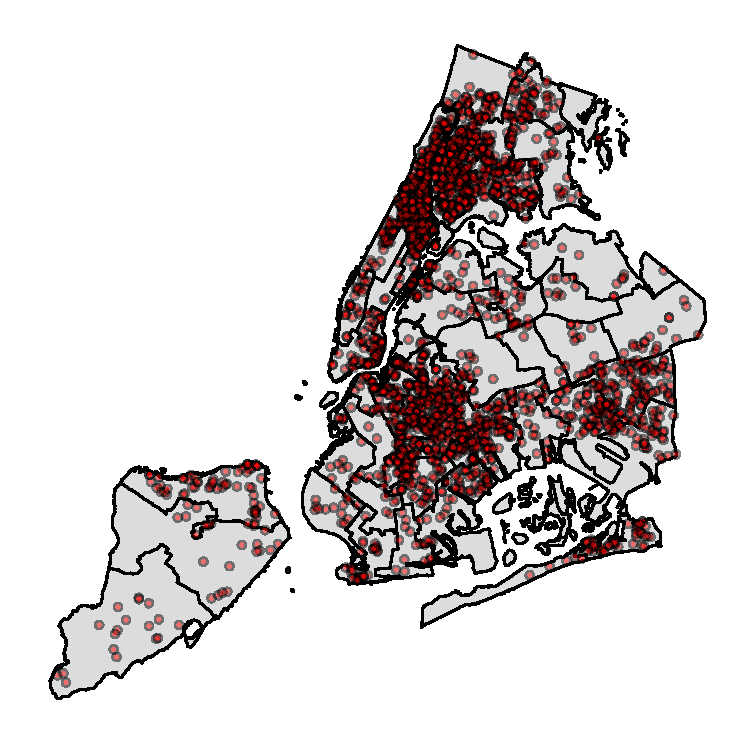
\includegraphics{UAR_submission_files/figure-latex/citywide-map-1} 

}

\caption{\label{fig:citymap}Lost Voters on Election Day, 2017}\label{fig:citywide-map}
\end{figure}

\input{"../../temp/table_whateverrrrr2.tex"}

\input{"../../temp/table2.tex"}
\begin{figure}[H]

{\centering 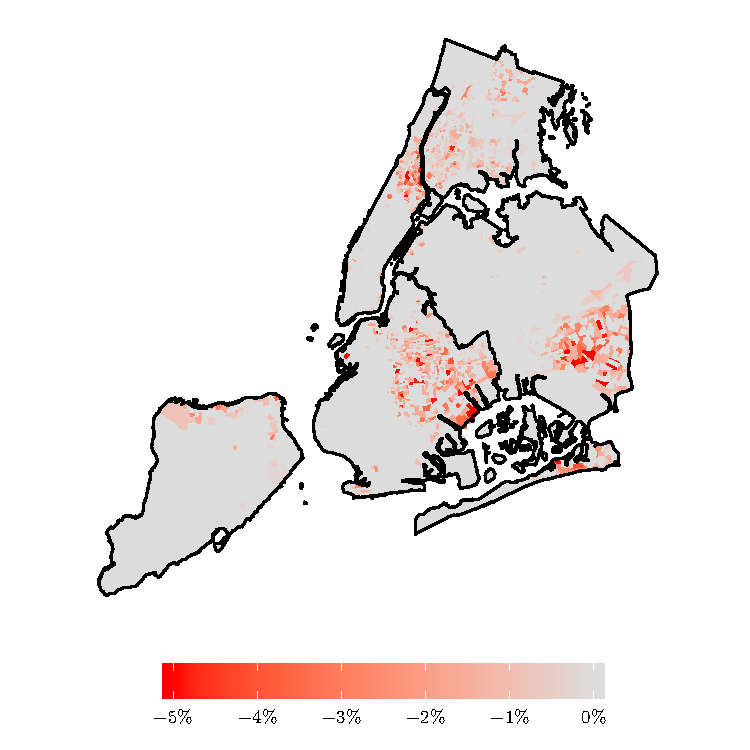
\includegraphics{UAR_submission_files/figure-latex/postest-map-1} 

}

\caption{\label{fig:postest}Estimated Depressive Effect of Felony Disenfranchisement}\label{fig:postest-map}
\end{figure}
\begin{table}[H]

\caption{\label{tab:block-table-chunk-did}\label{tab:did-match} Results of Block Group-Level Matching}
\centering
\resizebox{\linewidth}{!}{
\fontsize{10}{12}\selectfont
\begin{tabular}[t]{lllllrrrr}
\toprule
\multicolumn{1}{c}{ } & \multicolumn{2}{c}{Means: Unmatched Data} & \multicolumn{2}{c}{Means: Matched Data} & \multicolumn{4}{c}{Percent Improvement} \\
\cmidrule(l{3pt}r{3pt}){2-3} \cmidrule(l{3pt}r{3pt}){4-5} \cmidrule(l{3pt}r{3pt}){6-9}
 & Treated & Control & Treated & Control & Mean Diff & eQQ Med & eQQ Mean & eQQ Max\\
\midrule
Stop-and-Frisk Encounters (Per 1,000 Residents) & 1.52 & 1.22 & 1.52 & 1.40 & 59.18 & 80.84 & 74.64 & 64.80\\
\% Latino & 0.35 & 0.24 & 0.35 & 0.35 & 98.18 & 93.37 & 91.90 & 83.66\\
\% Non-Hispanic Black & 0.33 & 0.15 & 0.33 & 0.33 & 98.29 & 94.91 & 93.59 & 86.37\\
\% Non-Hispanic White & 0.20 & 0.41 & 0.20 & 0.20 & 97.57 & 92.56 & 89.24 & 83.47\\
Median Income & 52,352.43 & 70,311.87 & 52,352.43 & 52,177.85 & 99.03 & 92.14 & 87.32 & 68.43\\
\% With Some College & 0.65 & 0.71 & 0.65 & 0.65 & 96.85 & 90.55 & 86.81 & 69.31\\
Median Age & 35.61 & 38.12 & 35.61 & 35.68 & 97.21 & 68.61 & 73.56 & 63.48\\
Registration Rate & 0.98 & 0.93 & 0.98 & 0.96 & 49.13 & 72.80 & 64.99 & 31.69\\
\% Democrats & 0.73 & 0.64 & 0.73 & 0.73 & 94.29 & 94.58 & 91.69 & 84.47\\
\% Noncitizen & 0.17 & 0.17 & 0.17 & 0.18 & 90.15 & 90.13 & 83.20 & 61.09\\
\bottomrule
\end{tabular}}
\end{table}

\input{"../../temp/table1111.tex"}
\begin{table}[H]

\caption{\label{tab:shift-dobs-chunk}\label{tab:change-dobs} Results of Shifting Birthdates}
\centering
\begin{tabular}[t]{cc}
\toprule
Group & \makecell[l]{Number of Matches Between\\DOCCS and Voter File Records}\\
\midrule
Actual Birthdate & 20,955\\
Birthdate + 35 Days & 105\\
Birthdate - 35 Days & 92\\
\bottomrule
\end{tabular}
\end{table}
\end{singlespace}
\pagebreak
\pagenumbering{arabic}

\hypertarget{introduction}{%
\section*{Introduction}\label{introduction}}
\addcontentsline{toc}{section}{Introduction}

The political history of the United States has been characterized by a general, if nonlinear, trend toward universal suffrage (see, for instance, Keyssar \protect\hyperlink{ref-Keyssar2009}{2009}). At the time of the nation's founding, access to the ballot box was restricted to landed White men; over the following two centuries, the franchise was greatly expanded. Today, voting rights are considered foundational aspects of full citizenship (United Nations General Assembly Resolution 2200 (XXI)). Despite the United State's march toward ever-more-inclusive systems of democracy, however, one large group of American citizens is formally barred from voting. In most of the United States, citizens convicted of felonies are at least temporarily prohibited from casting ballots in elections (Justice \protect\hyperlink{ref-bcj_laws}{2019}). Although some states such as Florida and Louisiana have gradually moved to dismantle their systems of felony disenfranchisement, an estimated 4.7 million American citizens remain disenfranchised (Uggen, Larson, and Shannon \protect\hyperlink{ref-sentencing_2016}{2016}).

This paper furthers our understanding of the political implications of felony disenfranchisement by investigating its indirect turnout effects at the local level in New York City's 2017 mayoral election. Using administrative data from the Department of Corrections and Community Supervision and the registered voter file, I redefine ``lost voters'' as disenfranchised individuals with a history of voting. I test the effect of lost voters on neighborhood turnout after controlling for general neighborhood exposure to the criminal justice system, allowing me to tease apart the effect of disenfranchisement from the bundled indirect effects of overpolicing. I demonstrate that the neighborhoods left behind by lost voters turned out at substantially lower rates than other similar neighborhoods --- and that there is likely a causal relationship at play.

Given the reality of economic and racial segregation, it should not be surprising that the effects of felony disenfranchisement are highly spatially concentrated. Data available from New York City shows that in 2017, 10 of the New York Police Department's 77 precincts were responsible for more than a quarter of all arrests for felony charges. Many scholars have detailed the impact of living in areas with high levels of police activity. Residents of such neighborhoods suffer from worse physical health (Sewell and Jefferson \protect\hyperlink{ref-Sewell2016}{2016}) and are more likely to suffer from anxiety and exhibit symptoms of trauma (Geller et al. \protect\hyperlink{ref-Geller2014}{2014}). The labor markets and social networks in neighborhoods with high levels of policing and incarceration are disrupted (Clear \protect\hyperlink{ref-Clear2008}{2008}), while concentrated policing has also been credited with having a ``chilling effect'' on neighborhoods' willingness to reach out for help to local governments (Lerman and Weaver \protect\hyperlink{ref-Lerman2013}{2013}). Perhaps most troubling of all, these effects are not concentrated in random neighborhoods; as Gelman, Fagan, and Kiss (\protect\hyperlink{ref-Gelman2007}{2007}) shows, for instance, New York's ``stop-and-frisk'' policy impacted Black and Latino New Yorkers at rates far higher than Whites, even after controlling for neighborhood variability and race-specific arrest rates. The result is a disenfranchised population that looks far different than the rest of the state: according to data from the New York State Department of Corrections and Community Supervision, 49.5\% of individuals who were incarcerated in December of 2018 were non-Hispanic Black, although the Census Bureau estimates that just 14.3\% of the citizen voting age population in the state is non-Hispanic Black.\footnote{Latinos are also over-represented among the incarcerated population, though not as dramatically: Latinos make up 14.1\% of the citizen voting age population and 22.9\% of the incarcerated population.}

Felony disenfranchisement policies are part of a criminal justice system that disproportionately impacts Black Americans living in certain communities. The neighborhood-specific implications of felony disenfranchisement, however, remain largely unstudied. A number of studies have explored the effect of imprisonment and disenfranchisement on later political participation (White \protect\hyperlink{ref-White2019}{2019}\protect\hyperlink{ref-White2019}{b}; Gerber et al. \protect\hyperlink{ref-Gerber2015}{2015}; Burch \protect\hyperlink{ref-Burch2011}{2011}). Others have looked at the spillover effects of disenfranchisement on eligible Black voters at the state level (Bowers and Preuhs \protect\hyperlink{ref-Bowers2009}{2009}; King and Erickson \protect\hyperlink{ref-King2016}{2016}). With the exception of Burch (\protect\hyperlink{ref-Burch2013}{2013}), however, little attention has been paid to the impact of felony disenfranchisement on political participation at the neighborhood level.

Improving upon this literature is of great importance when we consider the spatial concentration of incarceration --- and, therefore, disenfranchisement. If the spillover effects of felony disenfranchisement are widely dispersed, the political consequences are likely similarly diffuse. If, however, the effects are both large enough to be detected at a statewide level (as the literature hints it might be) but also concentrated in a few neighborhoods, disenfranchisement laws likely severely undermine local political representation. This lowered participation can disadvantage neighborhoods insofar as they have unique candidate preferences (Kinsella, McTague, and Raleigh \protect\hyperlink{ref-Kinsella2015}{2015}). It could also lower the resources distributed to these neighborhoods, as politicians determine that too few votes can be won through investing in these areas (Martin \protect\hyperlink{ref-Martin2003}{2003}; Martin and Claibourn \protect\hyperlink{ref-Martin2013}{2013}). This is not merely of theoretical concern: research indicates that turnout differentials at the city level have material consequences. As Hajnal (\protect\hyperlink{ref-Hajnal2009}{2009}) tells us: ``low {[}and uneven{]} turnout results in losses in mayoral elections, less equitable racial and ethnic representation on city councils, and spending policies that are less in line with the preferences of racial and ethnic minorities and other disadvantaged groups'' (p.~8).

\hypertarget{literature-on-the-indirect-effects-of-felony-disenfranchisement}{%
\section*{Literature on the Indirect Effects of Felony Disenfranchisement}\label{literature-on-the-indirect-effects-of-felony-disenfranchisement}}
\addcontentsline{toc}{section}{Literature on the Indirect Effects of Felony Disenfranchisement}

A number of recent papers have attempted to estimate the indirect effects of felony disenfranchisement on turnout. These papers have generally looked for effects at the state level, and have come to different conclusions. King and Erickson (\protect\hyperlink{ref-King2016}{2016}), for instance, leverages state-level variation in disenfranchisement laws to estimate the impact that felony disenfranchisement has on turnout among Black Americans. They use data from the 2004 Current Population Survey Voting and Registration Supplement to calculate statewide turnout rates, and include estimates of the share of Black Americans who are disenfranchised in each state from Manza and Uggen (\protect\hyperlink{ref-locked_out}{2008}) to explore the impact of these policies on eligible voters. They conclude that disenfranchisement has large spillover effects for Black voters: where more Black residents are disenfranchised, eligible Black voters are less likely to cast a ballot. These findings are in line with other research that has explored whether the effects of disenfranchisement extend beyond those whose voting rights are directly suspended (Bowers and Preuhs \protect\hyperlink{ref-Bowers2009}{2009}; Ochs \protect\hyperlink{ref-Ochs2006}{2006}). As Bowers and Preuhs (\protect\hyperlink{ref-Bowers2009}{2009}) sums up: ``{[}I{]}t is not solely the direct vote of ex-felons that is denied through these laws. {[}Felony disenfranchisement{]} impacts the political power of communities that extends beyond felons' collateral penalty'' (p.~724).

Miles (\protect\hyperlink{ref-Miles2004}{2004}), however, leverages a triple-differences framework to investigate whether felony disenfranchisement reduces participation at the state level. This paper is more methodologically sophisticated than other research in this body of literature, and Miles (\protect\hyperlink{ref-Miles2004}{2004}) finds little-to-no effect from felony disenfranchisement on statewide turnout. The statewide research is thus in conflict --- it is unclear that felony disenfranchisement has a big enough effect on turnout to be detected at the state level. Despite its methodological improves, Miles (\protect\hyperlink{ref-Miles2004}{2004}) (like the other literature looking for statewide disenfranchisement turnout effects) uses the total disenfranchised population in each state, without disentangling the disenfranchised voters who would have voted in the absence of the policy from those who would not have.

Research looking for the effect of felony disenfranchisement in statewide statistics is fundamentally flawed. This approach is generally taken more for methodological reasons (disenfranchisement policies vary between but not within states) or practical reasons (national data at lower geographic levels about incarceration and voting patterns is difficult to find), but not for theoretical ones. The effects of incarceration --- and, therefore, felony disenfranchisement --- are not uniformly distributed throughout a given state; if felony disenfranchisement reduces turnout, it is likely to do so in geographically concentrated ways. Voting is a social act, and social networks play an important role in predicting political participation (e.g.~Foladare \protect\hyperlink{ref-Foladare1968}{1968}; Huckfeldt \protect\hyperlink{ref-Huckfeldt1979}{1979}; Kenny \protect\hyperlink{ref-Kenny1992}{1992}; Mutz \protect\hyperlink{ref-Mutz2002}{2002}). Literature from urban sociology has established that social networks are largely spatially bounded, and that local social ties are more important in lower-income neighborhoods (Guest and Wierzbicki \protect\hyperlink{ref-Guest1999}{1999}; Dawkins \protect\hyperlink{ref-Dawkins2006}{2006}). It should be no surprise, then, that neighborhoods have been shown to mobilize and demobilize voters through mechanisms above-and-beyond individual characteristics (Gimpel, Dyck, and Shaw \protect\hyperlink{ref-Gimpel2004}{2004}; Cho, Gimpel, and Dyck \protect\hyperlink{ref-Cho2006}{2006}). This is also the level at which any effect from felony disenfranchisement should theoretically operate.

The little research looking for turnout effects at the local level, however, is similarly conflicting. Burch (\protect\hyperlink{ref-Burch2013}{2013}), for instance, demonstrates that block groups in North Carolina with higher levels of incarceration had lower turnout. White (\protect\hyperlink{ref-White2019a}{2019}\protect\hyperlink{ref-White2019a}{a}), on the other hand, finds that incarceration has only moderate indirect effects on voting. She finds ``evidence of a short-term demobilization effect for people who see household members convicted or jailed in the weeks before the election, but no evidence of a lasting turnout effect from these experiences'' (p.~607). Neither of these papers, however, account for felony disenfranchisement laws \emph{per se}, but rather test the bundled indirect effects of proximal contact with incarceration (inclusive of disenfranchisement). Disenfranchised individuals who would not have voted in the absence of their incarceration are not directly affected by disenfranchisement policy; any indirect turnout effects associated with their incarceration, therefore, cannot be attributed to disenfranchisement policy.

This study addresses with both problems with the existing literature. I deal with geographic concentration by testing the relationship between felony disenfranchisement and turnout at the Census block group level. Secondly, I do not look for the indirect effects of proximal contact with \emph{any} individual incarcerated or paroled; rather, I test the relationship between neighborhood turnout and the disenfranchisement of an individual \emph{with a demonstrated history of voting}. As Gerber, Green, and Shachar (\protect\hyperlink{ref-Gerber2003}{2003}) and others indicate, past turnout is a very strong predictor of future turnout. Thus, by defining lost voters as individuals who previously participated, I can identify the individuals most likely to vote in the absence of felony disenfranchisement laws --- and therefore the individuals (and neighborhoods) most directly impacted by these laws. Although data on neighborhood incarceration rates is not available, I decompose the effect of disenfranchisement from the bundled treatments of exposure to the carceral state by controlling for neighborhood police stop rates.

\hypertarget{data}{%
\section*{Data}\label{data}}
\addcontentsline{toc}{section}{Data}

\hypertarget{criminal-justice-data}{%
\subsection*{Criminal Justice Data}\label{criminal-justice-data}}
\addcontentsline{toc}{subsection}{Criminal Justice Data}

The primary criminal justice dataset comes from a public records request filed with the New York State Department of Corrections and Community Supervision (NYSDOCCS). These records include individual-level incarceration and parole records for individuals who have been incarcerated in New York State since 1990. The data includes a host of information, including: first, middle, and last name; date of birth; class of offense; incarceration start and end dates; dates of parole; sex; race; and others.

The state makes records available only for individuals who have been incarcerated for felony offenses. It does not make information about individuals sentenced to probation or incarcerated for misdemeanors. Thus, while the data covers all individuals subject to felony disenfranchisement rules (only individuals incarcerated for felony offenses lose their voting rights), it limits the availability of a potentially helpful control group. It does not include individuals who are held in federal prisons; however, because the vast majority of incarcerated felons are held in state prisons, this is unlikely to affect the analysis.

\hypertarget{voter-file-data}{%
\subsection*{Voter File Data}\label{voter-file-data}}
\addcontentsline{toc}{subsection}{Voter File Data}

Most states in the United States are required to maintain files with information on all registered voters. In New York, this information is publicly available from the Board of Elections. It includes information on all registered voters, including: first, middle, and last name; date of birth; vote history; and other information. The New York State Voter File also includes information on voters who were previously registered but have since been purged, either because they moved, died, or were incarcerated for a felony offense. I use a snapshot of the registered voter file from April 30\textsuperscript{th}, 2018.

The New York State Voter File is unique in its treatment of ``purged'' voters: although most states remove voters from their voter files once they are no longer eligible to vote, New York continues to include them in the file (but marks them as purged). I can therefore identify voters who were registered in the past but have since been purged due to a felony conviction.

Further discussion about how these administrative records are linked and geocoded can be found in the Supplemental Information.

\hypertarget{research-design-and-expectations}{%
\section*{Research Design and Expectations}\label{research-design-and-expectations}}
\addcontentsline{toc}{section}{Research Design and Expectations}

I begin with an ordinary least squares regression estimated at the block group level. In this regression, neighborhood turnout is the dependent variable, while the number of lost voters is the independent variable of interest. I look at the 2017 mayoral election in New York City, and define a ``lost voter'' as an individual incarcerated or on felony parole on Election Day in 2017 who cast a ballot sometime between 2007 and 2016. Although the 2017 mayoral election was a low turnout contest, Hajnal (\protect\hyperlink{ref-Hajnal2009}{2009}) argues that these low turnout local elections are precisely where differential turnout rates can have the biggest consequences.

A regression that looks at turnout only in one year can shed little light on the causal effect of felony disenfranchisement. After investigating whether neighborhoods with lost voters turned out at lower rates in 2017, I use data from the 2016 presidential election to ask whether the loss of a voter leads to depressed turnout. I limit the pool of block groups to block groups with no lost voters in 2016, and test whether neighborhoods that had a lost voter one year later saw turnout decrease relative to their own history in 2016, and the 2017 turnout of neighborhoods that did not lose a voter in that period. Treated neighborhoods --- neighborhoods that lost a voter between the 2016 and 2017 elections --- are genetically matched to untreated neighborhoods. The matching procedure ensures that, prior to treatment, treated and control observations are substantially similar to one another based on observable characteristics.

I expect that neighborhoods with lost voters turned out at lower rates in 2017, and that the loss of a voter to felony disenfranchisement causes neighborhood turnout to decline. I expect these effects to operate through three primary mechanisms:

\begin{itemize}
\item
  Firstly, lost voters are likely members of families and communities where voting is valued. Because voting is a social act, incarcerated individuals who have participated in the past likely have family members who also vote. Proximal contact with an incarcerated individual can only have a depressive effect among eligible individuals who would have voted in the absence of the contact. Lost voters are more likely to be in relationship with individuals who would likely vote --- and who therefore can have their turnout depressed.
\item
  Secondly, would-be voters can encourage their family members and neighbors to go to the polls on Election Day. The removal of an individual who would provide social pressure to vote can reduce the sociality of voting for others and reduce their likelihood of voting.
\item
  Thirdly, proximal contact with voters who are imprisoned might change attitudes toward the state more dramatically than proximal contact with nonvoting individuals who are incarcerated. Voters are widely considered to be upholding their civic duty through participation; the incarceration of an engaged, dutiful citizen has the potential to change an eligible voter's perception of the state and democratic participation more than the incarceration of an individual who was not actively engaged through voting.
\end{itemize}

\hypertarget{results}{%
\section*{Results}\label{results}}
\addcontentsline{toc}{section}{Results}

Figure \ref{fig:citymap} shows where lost voters lived before going to prison, with city council districts also included. There were 2,518 such lost voters within New York City as of the 2017 general election.

FIGURE \ref{fig:citymap} ABOUT HERE

Although 73,223 individuals were formally disenfranchised as of the 2017 election, there were just 6,166 disenfranchised voters statewide who had participated in the past 10 years.\footnote{Because address prior to incarceration is not available for individuals who were not registered to vote, computing the total number of formally disenfranchised individuals in New York City is not possible.} Just 8.4\% of formally disenfranchised individuals, therefore, were individuals with a demonstrated history of participating.

The spatial concentration of lost voters is readily apparent. In some communities, such as Greenwich Village and Brooklyn Heights, hardly any voters were disqualified from participating in the 2017 elections. In other communities, such as Harlem and Central Brooklyn, large numbers of past voters were not allowed to cast a ballot for mayor.

Table \ref{tab:demos} demonstrates just how different the neighborhoods with lost voters are from the rest of the city. The first column in Table \ref{tab:demos} weights the chacteristics of each block group in the city by its population; the second column weights the block groups by their number of lost voters. The median income in neighborhoods with lost voters is less than three-quarters that of unaffected neighborhoods. The average lost voter came from a neighborhood that was nearly twice as Black as the city as a whole; their neighborhoods were also home to a far larger share of Democratic voters than other neighborhoods. Unsurprisingly, lost voters also came from neighborhoods with 60\% more police stops than the citywide average.

TABLE \ref{tab:demos} ABOUT HERE

\hypertarget{testing-for-neighborhood-turnout-differences}{%
\subsection*{Testing for Neighborhood Turnout Differences}\label{testing-for-neighborhood-turnout-differences}}
\addcontentsline{toc}{subsection}{Testing for Neighborhood Turnout Differences}

I begin by asking whether turnout was lower in the 2017 mayoral election in neighborhoods with lost voters. Block group turnout rates are calculated using the geocoded voter file. Each voter's record indicates whether the voter participated in the 2017 general election. These records are then aggregated to estimate the number of ballots cast in each neighborhood. The number of ballots cast is divided by the neighborhood's citizen voting age population (CVAP, estimated by the Census Bureau). The independent variable of interest measures the number of lost voters in a neighborhood.

I also control for other social and political indicators: neighborhood racial characteristics, median income, education, age, population, and share noncitizen\footnote{The Census Bureau does not make noncitizen estimates available at the block group level. As such, block groups are assigned their census tract's share noncitizen for matching purposes.} come from the Census Bureau's 2017 5-year American Community Survey estimates. Party affiliation rates come from the geocoded voter file. Registration rate is calculated by dividing the number of registered voters (calculated using the voter file) by the CVAP. I include voteshare won by the winning city council representative in 2017 as a proxy for the competitiveness of the local race;\footnote{Where neighborhoods cross council district lines, this measure is the mean competitiveness faced by each voter in the neighborhood} where city council district races were more competitive, I expect that more voters will have turned out.

To completely decompose the effects of disenfranchisement from incarceration more generally, we would need to control for the number of incarcerated or paroled individuals in a neighborhood. If, after controlling for a neighborhood's general exposure to incarceration, there was a negative turnout effect from the loss of a voter, that loss could be attributed to disenfranchisement.

Unfortunately, such data does not exist; the State of New York does not make pre-incarceration addresses available to the public. In its place, I use data from the NYPD on stop-and-frisk encounters with the police. These models include the number of times residents were stopped by the police from January -- October of 2017. This is intended to control for general neighborhood exposure to the carceral state.

Much of the literature has discussed whether felony disenfranchisement is particularly demobilizing for eligible Black voters. Model 2, therefore, interacts the number of lost voters with the share of the block group that is non-Hispanic Black.

Table \ref{tab:trad-reg} presents the results of ordinary least squares regressions testing neighborhood turnout rates in 2017. Robust standard errors are clustered by city council district.\footnote{Where neighborhoods cross city council district lines, they are assigned the district in which most of their voters live for clustering purposes.}

TABLE \ref{tab:trad-reg} ABOUT HERE

The results presented in Table \ref{tab:trad-reg} indicate that neighborhoods with lost voters turned out at lower rates in the 2017 election. Each missing voter in a block group reduces that neighborhood's turnout by about 0.8 percentage points. Model 2, however, makes clear that this effect is concentrated in Black neighborhoods. In neighborhoods where most residents are Black, each lost voter is associated with a turnout decrease of up to 1.93 percentage points. The neighborhoods most affected by felony disenfranchisement are neighborhoods where incarceration patterns overlap with Black communities.

The block groups where these depressive effects are concentrated are not randomly distributed throughout the city. They are highly spatially concentrated in Central Brooklyn, Eastern Queens, and Harlem. Figure \ref{fig:postest} applies the coefficient on \(Lost\ Voters \times Share\ Black\) from Model 2 in Table \ref{tab:trad-reg} to the city's block groups. The estimated depressive effect is \(-0.019\times Lost\ Voters \times Share\ Black\).

FIGURE \ref{fig:postest} ABOUT HERE

\hypertarget{toward-a-causal-estimate}{%
\subsection*{Toward a Causal Estimate}\label{toward-a-causal-estimate}}
\addcontentsline{toc}{subsection}{Toward a Causal Estimate}

As the analysis above make clear, neighborhoods with lost voters saw substantially lower turnout in the 2017 mayoral election than neighborhoods without lost voters. The possibility remains, however, that treated neighborhoods systematically differ from untreated neighborhoods in ways that cannot be accounted for using the available data. Moreover, by looking at turnout from just one election, the best we could hope to uncover is a correlation between disenfranchisement and turnout. Uncovering the causal effect requires looking across elections (or the very strong assumptions that all relevant neighborhood characteristics are accounted for).

In order to estimate the causal effect of felony disenfranchisement on neighborhood-level turnout, I now test whether losing a voter between the 2016 and 2017 elections resulted in decreased turnout in 2017. I begin by restricting the set of neighborhoods to only neighborhoods that had no lost voters on election day in 2016. This process is the inverse of the process described above: I identify all individuals who were in prison or on parole on November 8\textsuperscript{th}, 2016, who had cast a ballot between 2006 and 2015. These individuals' home neighborhoods are removed from the subsequent analysis. I then identify the neighborhoods that did have lost voters in 2017; these block groups are our ``treated'' block groups, while the neighborhoods with lost voters in neither 2016 nor 2017 serve as our controls.

Of course, as demonstrated in Table \ref{tab:demos}, neighborhoods with lost voters are very different than neighborhoods without lost voters. Control and treatment neighborhoods might have different levels of turnout in 2017 even in the absence of felony disenfranchisement. To account for this possibility, I use a genetic matching model (Sekhon \protect\hyperlink{ref-Sekhon2011}{2011}) to match each treated block group to one untreated block group, using the same characteristics detailed in Table \ref{tab:trad-reg} but based on their 2016 characteristics. Matched ties are not broken, leaving the potential for some treated block groups to match to more than one control; the observations are weighted accordingly. Only treated block groups and the untreated block groups with which they match --- the controls --- are retained.

Although it may seem counterintuitive to discard some potential control block groups, doing so gives us a major advantage: it allows us to conceptualize the ``treatment'' (the loss of a voter) as a natural experiment. Because the treatment and control groups look similar based on their observable 2016 characteristics, the treatment can be understood as quasi-randomly assigned.

Table \ref{tab:did-match} presents the results of matching on these subsets of neighborhoods. The matching procedure substantially improves the similarly between treated and control block groups along all characteristics. Table \ref{tab:did-match} mirrors Table \ref{tab:demos} above: treated neighborhoods are far less White, had many more stop-and-frisk encounters, and had much lower median incomes.

TABLE \ref{tab:did-match} ABOUT HERE

In Table \ref{tab:did-reg}, I present the outcome of an OLS regression on this subset of block groups. The variable \emph{D(2017)} tests whether turnout for control block groups declined in 2017 relative to 2016. I test whether there was a difference in turnout between control and treatment neighborhoods in 2016 with \emph{D(Treat)}. Of most interest is the coefficient on \emph{D(Treat) \(\times\) D(2017)}, which tests whether turnout decreased more from 2016 to 2017 in treated block groups than in the controls. Model 1 includes only these covariates (and fixed effects for Congressional district to account for potential differences in competitiveness in 2016), while Model 2 also includes the variables that were used for the matching procedure. Since each neighborhood appears in the panel twice --- once in 2016, and once in 2017 --- each observation takes the characteristics of the year in which it appears. This is especially important for the stop-and-frisk variable: Model 2 specifically controls for the possibility that police activity increased more in treated neighborhoods in 2017. Model 3 adds block group-level fixed effects to Model 2 in order to control for time-invariant neighborhood characteristics. Robust standard errors are clustered at the level of the match (Abadie and Spiess \protect\hyperlink{ref-Abadie2019}{2019}).

TABLE \ref{tab:did-reg} ABOUT HERE

Table \ref{tab:did-reg} makes clear that the removal of lost voters likely has a causal effect on neighborhoods' turnout rates. In each specification, turnout decreased from 2016 to 2017 in treated neighborhoods by at least 2.6 percentage points more than in untreated neighborhoods. It is worth noting that this is the treatment effect on the treated --- which is to say, it is estimated using only the 319 neighborhoods with no lost voters in 2016 who lost one in the subsequent year. These neighborhoods may differ from neighborhoods that had lost voters in both 2016 and 2017. The marginal effect of a lost voter could be lower in neighborhoods that consistently have lost voters and thus have less to ``learn'' about the state from the loss of any one individual to incarceration. Neighborhoods that consistently have lost voters are more likely to be the places most impacted by felony disenfranchisement. Among block groups that had a lost voter in 2017, those who had no lost voters in 2016 were higher-income (\$51k versus \$56k), had higher shares non-Hispanic White (16\% versus 21\%), a lower share non-Hispanic Black (39\% versus 32\%), and a smaller share were registered as Democrats (76\% versus 73\%).\footnote{Each of these differences are significant at the 99\% confidence level.}

Of particular note is the lower share of the population in these neighborhoods that is Black. The analyses above indicate that neighborhoods with more Black residents respond the most strongly to felony disenfranchisement. The set of neighborhoods in this section, therefore, are likely among the least likely to see this relationship. Nevertheless, that this relationship can be detected at the block group level lends credence to the causal relationship between lost voters and depressed turnout.

\hypertarget{discussion}{%
\section*{Discussion}\label{discussion}}
\addcontentsline{toc}{section}{Discussion}

During the 2017 mayoral election, felony disenfranchisement laws were responsible for removing an estimated 2,518 voters from New York City neighborhoods. The spatial concentration of these lost voters is striking, as demonstrated in Figure \ref{fig:citywide-map}, and the systematic removal of voters from these neighborhoods is troubling. However, more than one million votes were cast in the general election of 2017. Although felony disenfranchisement rules have implications for the individuals targeted by them, the removal of such a small number of voters --- concentrated though they are --- is unlikely to have large direct effects on turnout and representation.

As this analysis makes clear, however, felony disenfranchisement reaches beyond the individuals who are incarcerated. Despite methodological problems, previous literature has hinted that felony disenfranchisement impacts Black turnout at the state level; this analysis demonstrates that these demobilizing effects intersect with geographical space to systematically depress the vote in neighborhoods where voters are being sent to prison. As discussed above, these neighborhoods have far lower incomes than the rest of the city: the median income of block groups without any lost voters is more than 40\% higher than the median income of block groups with lost voters. Similarly, just 17\% of individuals in the average block group with a lost voter were White, compared with 40\% of the population in other block groups. Felony disenfranchisement has spillover effects on neighborhood turnout, and these neighborhoods systematically differ from the rest of the city's population. The effects are concentrated in neighborhoods where the most marginalized members of society live. These highly concentrated spillover effects are cause for major concern.

Of equal concern is the apparent concentration of these effects in Black neighborhoods. Table \ref{tab:trad-reg} indicates that once the lost voter indicator is interacted with the share of a neighborhood that is non-Hispanic Black, the lost voter indicator is nonsignificant. This means that lost voters have little spillover effects in neighborhoods with small Black populations. Understanding the magnitude of this finding is important. In New York City, there are 1,386 block groups where the Black community makes up more than 38\% of the population (the average for treated block groups), with an average of 912 voting age citizens. Model 2 of Table \ref{tab:trad-reg} indicates that, in a block group that is 38\% Black with a citizen voting age population of 912, having any lost voter reduced turnout by 6.7 ballots. Conversely, in a block group with the same voting age population that is just 16\% Black (the average for untreated block groups), the loss of any voter decreased turnout by just 1.7 ballots --- hardly more votes than the lost voter herself.

Why do lost voters in Black neighborhoods have such large spillover effects, when lost voters in predominantly non-Black neighborhoods do not? Much of the previous literature in this space establishes that individuals who have negative interactions with the government are less likely to choose to interact with the state in the future --- that these interactions have large ``interpretive effects'' (Pierson \protect\hyperlink{ref-Pierson1993}{1993}). Lerman and Weaver (\protect\hyperlink{ref-Lerman2013}{2013}), for instance, shows that neighborhoods where there are many police stops that involve searches or use of force use 311 services less frequently. Weaver and Lerman (\protect\hyperlink{ref-Weaver2010}{2010}) argues that interactions with the criminal justice system changes how individuals understand both their identities as citizens and the nature of governmental structures. Similarly, Lerman and Weaver (\protect\hyperlink{ref-Lerman2014}{2014}) tells us that those who have had contact with the criminal justice system consider political participation not just unfruitful but rather ``as something to be actively avoided'' (p.~16). It is perhaps unsurprising that the negative spillover effects are largest in neighborhoods where criminal justice involvement is most keenly (and unfairly) felt; namely, in plurality and majority Black neighborhoods.

Individuals who live in neighborhoods where police activity is relatively limited may interpret the incarceration of a neighbor as a largely individual phenomenon. If it is understood as an isolated or individual event, voters in these neighborhoods who are not incarcerated are not likely to update their view of the state. They may draw no connections between their neighbor's imprisonment and their own efficacy as a voter. In the neighborhoods where policing is most prevalent --- often, lower-income Black communities --- the incarceration of a neighbor might not be interpreted so individualistically. It may, rather, be interpreted as another reminder of the government's unfairness. If a would-be voter finds herself soured on political participation because of her neighbor's incarceration, she may be less likely to cast a ballot.

A large body of research indicates that, even after controlling for various sociodemographic characteristics and interactions with the police, Black Americans have far more negative views of the criminal justice system than White Americans (e.g.~Browning and Cao \protect\hyperlink{ref-Browning1992}{1992}; Hurwitz and Peffley \protect\hyperlink{ref-Hurwitz2005}{2005}; Henderson et al. \protect\hyperlink{ref-Henderson1997}{1997}; Wu, Sun, and Triplett \protect\hyperlink{ref-Wu2009}{2009}). Experience with the criminal justice system is less likely to be viewed in isolation (and therefore more likely to affect voting patterns) in Black neighborhoods. There is therefore strong reason to suspect that the concentrated depressive effects of felony disenfranchisement in Black neighborhoods arise from these distinct interpretations of the act of incarceration by the state.

Ultimately, the analysis at hand cannot answer the causal mechanism for these depressive effects, or why the depressive effect is concentrated in Black neighborhoods. As Walker (\protect\hyperlink{ref-Walker2020}{2020}) notes, ``contextual measures of proximity do not accurately assess the relational aspect central to the concept of proximal contact'' (p.~123). Administrative data can only get us so far. Other research designs are necessary to investigate how neighbors understand the incarceration of their neighbors, how they react on voting day, and whether these effects are racially moderated. Much of the work being done by Hannah Walker and coauthors (Walker \protect\hyperlink{ref-Walker2014}{2014}, \protect\hyperlink{ref-Walker2020}{2020}; Walker and García-Castañon \protect\hyperlink{ref-Walker2017}{2017}) does point to racial differences in political responses to proximal contact with systems of incarceration.

This paper uncovers surprisingly large effects. It is possible that, despite controlling for neighborhood exposure to the carceral state using stop-and-frisk data, the analysis cannot entirely decompose the effect of disenfranchisement from the bundled experience of seeing a neighbor go to prison. Future research must gather better data on local patterns of incarceration in order to better distinguish turnout patterns in neighborhoods where voters are sent to prison from neighborhoods where non-voters are incarcerated. Future work should similarly test whether these effects, identified in a relatively uncompetitive local election, are also present in competitive and national elections.

For decades, scholars have detailed the problems associated with poor and segregated urban neighborhoods (Wilson \protect\hyperlink{ref-Wilson1990}{1990}). More recent work has begun to interrogate the ways in which the increasing reach of the carceral state shapes the economic and political behavior of individuals caught up in the criminal justice system and their community members. Much of this work, however, has focused on either the impacts of living in marginalized communities (by measuring health and economic impacts) or has not accounted for the importance of physical space (by focusing only on proximal social, and not geographic, contact with directly impacted individuals). This analysis allows us to understand the implications for living in a neighborhood where individuals likely to cast a ballot are not allowed to because of a felony conviction. I find that neighborhoods that are home to lost voters --- and particularly neighborhoods with large Black populations --- systematically turn out for local elections at lower rates than otherwise similar neighborhoods.

This has major ramifications for how we understand the political positioning of the minority neighborhoods most impacted by overpolicing and incarceration. In the case of the 2017 election, there were likely no electoral consequences: Bill de Blasio won reelection handily, and neighborhoods with lost voters overwhelmingly supported his candidacy. A lack of electoral consequences in 2017, however, should not be interpreted to mean that the disparate and concentrated depressive effects of felony disenfranchisement never have implications for who is elected to local office. As Hajnal and Trounstine (\protect\hyperlink{ref-Hajnal2005}{2005}) shows, racial turnout differentials can have real consequences for city politics.

Moreover, we cannot conclude that depressed turnout in these neighborhoods in 2017 had no impact on their representation. City council members representing these neighborhoods, for instance, may determine that pushing for policies popular with these constituents (such as stricter police oversight) will not garner enough votes to make such a fight worthwhile. Although spillover effects from felony disenfranchisement may not have changed who won power in 2017, it very possibly altered how those individuals \emph{held} and \emph{used} their power.

Felony disenfranchisement laws, originally adopted during Jim Crow, have taken on a new life in the era of mass incarceration. Abundant research has demonstrated the pernicious ways in which overincarceration dogs the lives of poor and non-White Americans. As this study shows, however, the neighborhoods bearing the brunt of felony disenfranchisement are also seeing their political power diminished through reduced turnout. The interlocking nature of racioeconomic segregation, policing patterns, and felony disenfranchisement all combine to undermine the political power of marginalized communities in New York City.

\newpage

\hypertarget{supplemental-information}{%
\section*{Supplemental Information}\label{supplemental-information}}
\addcontentsline{toc}{section}{Supplemental Information}

I here present more information on how the full data set used in the body of this paper was constructed.

\hypertarget{geocoding}{%
\subsection*{Geocoding}\label{geocoding}}
\addcontentsline{toc}{subsection}{Geocoding}

Voters' home addresses were converted to latitudes and longitudes using a geocoder provided by SmartyStreets. I then used the statistical software R to map these latitudes and longitudes to census block groups, census tracts, and city council districts using shapefiles publicly available from the Census Bureau and the City of New York. This geocoder is not perfect: among individuals registered to vote in New York City, the geocoder failed to determine the latitude and longitude of the addresses of 1\% of registered voters. The geocoder was slightly less successful when it came to lost voters (defined and discussed below); 1.6\% of these individuals were not geocoded. Voters who were not successfully geocoded are dropped from the dataset; however, because so few observations went uncoded, it is unlikely to affect the analysis.

\hypertarget{matching}{%
\subsection*{Matching}\label{matching}}
\addcontentsline{toc}{subsection}{Matching}

I construct the primary dataset by matching the administrative criminal supervision records with the registered voter file. I match using first, middle, and last names, as well as dates of birth. Capitalization in names in both datasets is standardized, and punctuation and spaces are removed. If a middle name is missing in one dataset but not in the other, I consider this a match. Similarly, if one dataset includes only a middle initial which matches to the first letter of the middle name the other data set, this is considered a match. First and last names, and dates of birth, must match exactly between the two datasets.

To test for false positive matches, I employ the test developed in Meredith and Morse (\protect\hyperlink{ref-Meredith2013}{2013}). I slightly alter the date of birth reported in the NYSDOCCS dataset to create false records. Comparing the number of matches between these ``fake'' records and the voter file with the number of matches between the ``true'' records and the voter file provides an estimate of how frequently false positives occur. Table \ref{tab:change-dobs} shows the results of true matches, as well as matches using a set of fake records created by adding or subtracting 35 days from an individual's birthdate. This analysis indicates that false positives account for between 0.4 and 0.5\% of all matches, a share that is likely too small to have any material impact on the overall analysis. The numbers in Table \ref{tab:change-dobs} are derived by matching (and modifying) all individuals who were incarcerated or on parole on Election Day in 2017 with the registered voter file from April of 2018.

TABLE \ref{tab:change-dobs} ABOUT HERE

Testing for false negatives is more challenging. If an individual marries and changes her name after being discharged from parole, for instance, I will not identify her using my matching methodology. For two reasons, however, false positives are unlikely to pose major challenges: firstly, women are far more likely to change their last names than men, and women make up barely 6\% of individuals who have been discharged from felony parole. Secondly, because both parolee discharge and voter registration are legal records, individuals are likely to be recorded using their full names (that is to say, an individual is unlikely to be ``Alex'' in one set of records and ``Alexander'' in the other).

\theendnotes

\newpage

\hypertarget{references}{%
\section*{References}\label{references}}
\addcontentsline{toc}{section}{References}

\hypertarget{refs}{}
\begin{cslreferences}
\leavevmode\hypertarget{ref-Abadie2019}{}%
Abadie, Alberto, and Jann Spiess. 2019. ``Robust Post-Matching Inference.'' \emph{Working Paper.}

\leavevmode\hypertarget{ref-Bowers2009}{}%
Bowers, Melanie, and Robert R. Preuhs. 2009. ``Collateral Consequences of a Collateral Penalty: The Negative Effect of Felon Disenfranchisement Laws on the Political Participation of Nonfelons*.'' \emph{Social Science Quarterly} 90 (3): 722--43. \url{https://doi.org/10.1111/j.1540-6237.2009.00640.x}.

\leavevmode\hypertarget{ref-Browning1992}{}%
Browning, Sandra Lee, and Liqun Cao. 1992. ``The Impact of Race on Criminal Justice Ideology.'' \emph{Justice Quarterly} 9 (4): 685--701. \url{https://doi.org/10.1080/07418829200091611}.

\leavevmode\hypertarget{ref-Burch2011}{}%
Burch, Traci. 2011. ``Turnout and Party Registration Among Criminal Offenders in the 2008 General Election.'' \emph{Law \& Society Review} 45 (3): 699--730. \url{https://doi.org/10.1111/j.1540-5893.2011.00448.x}.

\leavevmode\hypertarget{ref-Burch2013}{}%
Burch, Traci R. 2013. ``Effects of Imprisonment and Community Supervision on Neighborhood Political Participation in North Carolina:'' \emph{The ANNALS of the American Academy of Political and Social Science}, November. \url{https://doi.org/10.1177/0002716213503093}.

\leavevmode\hypertarget{ref-Cho2006}{}%
Cho, Wendy K. Tam, James G. Gimpel, and Joshua J. Dyck. 2006. ``Residential Concentration, Political Socialization, and Voter Turnout.'' \emph{The Journal of Politics} 68 (1): 156--67. \url{https://doi.org/10.1111/j.1468-2508.2006.00377.x}.

\leavevmode\hypertarget{ref-Clear2008}{}%
Clear, Todd R. 2008. ``The Effects of High Imprisonment Rates on Communities.'' \emph{Crime and Justice} 37 (1): 97--132. \url{https://doi.org/10.1086/522360}.

\leavevmode\hypertarget{ref-Dawkins2006}{}%
Dawkins, Casey J. 2006. ``Are Social Networks the Ties That Bind Families to Neighborhoods?'' \emph{Housing Studies} 21 (6): 867--81. \url{https://doi.org/10.1080/02673030600917776}.

\leavevmode\hypertarget{ref-Foladare1968}{}%
Foladare, Irving S. 1968. ``The Effect of Neighborhood on Voting Behavior.'' \emph{Political Science Quarterly} 83 (4): 516--29. \url{https://doi.org/10.2307/2146812}.

\leavevmode\hypertarget{ref-Geller2014}{}%
Geller, Amanda, Jeffrey Fagan, Tom Tyler, and Bruce G. Link. 2014. ``Aggressive Policing and the Mental Health of Young Urban Men.'' \emph{American Journal of Public Health} 104 (12): 2321--7. \url{https://doi.org/10.2105/AJPH.2014.302046}.

\leavevmode\hypertarget{ref-Gelman2007}{}%
Gelman, Andrew, Jeffrey Fagan, and Alex Kiss. 2007. ``An Analysis of the New York City Police Department's `Stop-and-Frisk' Policy in the Context of Claims of Racial Bias.'' \emph{Journal of the American Statistical Association} 102 (479): 813--23. \url{https://doi.org/10.1198/016214506000001040}.

\leavevmode\hypertarget{ref-Gerber2003}{}%
Gerber, Alan S., Donald P. Green, and Ron Shachar. 2003. ``Voting May Be Habit-Forming: Evidence from a Randomized Field Experiment.'' \emph{American Journal of Political Science} 47 (3): 540--50. \url{https://doi.org/10.1111/1540-5907.00038}.

\leavevmode\hypertarget{ref-Gerber2015}{}%
Gerber, Alan S., Gregory A. Huber, Marc Meredith, Daniel R. Biggers, and David J. Hendry. 2015. ``Can Incarcerated Felons Be (Re)Integrated into the Political System? Results from a Field Experiment.'' \emph{American Journal of Political Science} 59 (4): 912--26. \url{https://doi.org/10.1111/ajps.12166}.

\leavevmode\hypertarget{ref-Gimpel2004}{}%
Gimpel, James G., Joshua J. Dyck, and Daron R. Shaw. 2004. ``Registrants, Voters, and Turnout Variability Across Neighborhoods.'' \emph{Political Behavior} 26 (4): 343--75. \url{https://doi.org/10.1007/s11109-004-0900-4}.

\leavevmode\hypertarget{ref-Guest1999}{}%
Guest, Avery M., and Susan K. Wierzbicki. 1999. ``Social Ties at the Neighborhood Level: Two Decades of GSS Evidence.'' \emph{Urban Affairs Review}, September. \url{https://doi.org/10.1177/10780879922184301}.

\leavevmode\hypertarget{ref-Hajnal2009}{}%
Hajnal, Zoltan. 2009. \emph{America's Uneven Democracy: Race, Turnout, and Representation in City Politics}. Cambridge ; New York: Cambridge University Press.

\leavevmode\hypertarget{ref-Hajnal2005}{}%
Hajnal, Zoltan, and Jessica Trounstine. 2005. ``Where Turnout Matters: The Consequences of Uneven Turnout in City Politics.'' \emph{The Journal of Politics} 67 (2): 515--35. \url{https://doi.org/10.1111/j.1468-2508.2005.00327.x}.

\leavevmode\hypertarget{ref-Henderson1997}{}%
Henderson, Martha L., Francis T. Cullen, Liqun Cao, Sandra Lee Browning, and Renee Kopache. 1997. ``The Impact of Race on Perceptions of Criminal Injustice.'' \emph{Journal of Criminal Justice} 25 (6): 447--62. \url{https://doi.org/10.1016/S0047-2352(97)00032-9}.

\leavevmode\hypertarget{ref-Huckfeldt1979}{}%
Huckfeldt, R. Robert. 1979. ``Political Participation and the Neighborhood Social Context.'' \emph{American Journal of Political Science} 23 (3): 579--92. \url{https://doi.org/10.2307/2111030}.

\leavevmode\hypertarget{ref-Hurwitz2005}{}%
Hurwitz, Jon, and Mark Peffley. 2005. ``Explaining the Great Racial Divide: Perceptions of Fairness in the U.S. Criminal Justice System.'' \emph{The Journal of Politics} 67 (3): 762--83. \url{https://doi.org/10.1111/j.1468-2508.2005.00338.x}.

\leavevmode\hypertarget{ref-bcj_laws}{}%
Justice, Brennan Center for. 2019. ``Criminal Disenfranchisement Laws Across the United States.'' \emph{Brennan Center for Justice}, May. \url{https://www.brennancenter.org/our-work/research-reports/criminal-disenfranchisement-laws-across-united-states}.

\leavevmode\hypertarget{ref-Kenny1992}{}%
Kenny, Christopher B. 1992. ``Political Participation and Effects from the Social Environment.'' \emph{American Journal of Political Science} 36 (1): 259--67. \url{https://doi.org/10.2307/2111432}.

\leavevmode\hypertarget{ref-Keyssar2009}{}%
Keyssar, Alexander. 2009. \emph{The Right to Vote: The Contested History of Democracy in the United States}. Revised edition. New York: Basic Books.

\leavevmode\hypertarget{ref-King2016}{}%
King, Bridgett A., and Laura Erickson. 2016. ``Disenfranchising the Enfranchised: Exploring the Relationship Between Felony Disenfranchisement and African American Voter Turnout.'' \emph{Journal of Black Studies}, July. \url{https://doi.org/10.1177/0021934716659195}.

\leavevmode\hypertarget{ref-Kinsella2015}{}%
Kinsella, Chad, Colleen McTague, and Kevin N. Raleigh. 2015. ``Unmasking Geographic Polarization and Clustering: A Micro-Scalar Analysis of Partisan Voting Behavior.'' \emph{Applied Geography} 62 (August): 404--19. \url{https://doi.org/10.1016/j.apgeog.2015.04.022}.

\leavevmode\hypertarget{ref-Lerman2013}{}%
Lerman, Amy E., and Vesla Weaver. 2013. ``Staying Out of Sight? Concentrated Policing and Local Political Action:'' \emph{The ANNALS of the American Academy of Political and Social Science}, November. \url{https://doi.org/10.1177/0002716213503085}.

\leavevmode\hypertarget{ref-Lerman2014}{}%
Lerman, Amy E., and Vesla M. Weaver. 2014. \emph{Arresting Citizenship: The Democratic Consequences of American Crime Control}. Chicago Studies in American Politics. Chicago ; London: The University of Chicago Press.

\leavevmode\hypertarget{ref-locked_out}{}%
Manza, Jeff, and Christopher Uggen. 2008. \emph{Locked Out: Felon Disenfranchisement and American Democracy}. Studies in Crime and Public Policy. New York: Oxford University Press.

\leavevmode\hypertarget{ref-Martin2003}{}%
Martin, Paul S. 2003. ``Voting's Rewards: Voter Turnout, Attentive Publics, and Congressional Allocation of Federal Money.'' \emph{American Journal of Political Science} 47 (1): 110--27. \url{https://doi.org/10.1111/1540-5907.00008}.

\leavevmode\hypertarget{ref-Martin2013}{}%
Martin, Paul S., and Michele P. Claibourn. 2013. ``Citizen Participation and Congressional Responsiveness: New Evidence That Participation Matters.'' \emph{Legislative Studies Quarterly} 38 (1): 59--81. \url{https://doi.org/10.1111/lsq.12003}.

\leavevmode\hypertarget{ref-Meredith2013}{}%
Meredith, Marc, and Michael Morse. 2013. ``Do Voting Rights Notification Laws Increase Ex-Felon Turnout?:'' \emph{The ANNALS of the American Academy of Political and Social Science}, November. \url{https://doi.org/10.1177/0002716213502931}.

\leavevmode\hypertarget{ref-Miles2004}{}%
Miles, Thomas J. 2004. ``Felon Disenfranchisement and Voter Turnout.'' \emph{The Journal of Legal Studies} 33 (1): 85--129. \url{https://doi.org/10.1086/381290}.

\leavevmode\hypertarget{ref-Mutz2002}{}%
Mutz, Diana C. 2002. ``The Consequences of Cross-Cutting Networks for Political Participation.'' \emph{American Journal of Political Science} 46 (4): 838--55. \url{https://doi.org/10.2307/3088437}.

\leavevmode\hypertarget{ref-Ochs2006}{}%
Ochs, Holona Leanne. 2006. ``\,`Colorblind' Policy in Black and White: Racial Consequences of Disenfranchisement Policy.'' \emph{Policy Studies Journal} 34 (1): 81--93. \url{https://doi.org/10.1111/j.1541-0072.2006.00146.x}.

\leavevmode\hypertarget{ref-Pierson1993}{}%
Pierson, Paul. 1993. ``When Effect Becomes Cause: Policy Feedback and Political Change.'' \emph{World Politics} 45 (4): 595--628. \url{https://doi.org/10.2307/2950710}.

\leavevmode\hypertarget{ref-Sekhon2011}{}%
Sekhon, Jasjeet S. 2011. ``Multivariate and Propensity Score Matching Software with Automated Balance Optimization: The Matching Package for R.'' \emph{Journal of Statistical Software} 42 (1): 1--52. \url{https://doi.org/10.18637/jss.v042.i07}.

\leavevmode\hypertarget{ref-Sewell2016}{}%
Sewell, Abigail A., and Kevin A. Jefferson. 2016. ``Collateral Damage: The Health Effects of Invasive Police Encounters in New York City.'' \emph{Journal of Urban Health} 93 (1): 42--67. \url{https://doi.org/10.1007/s11524-015-0016-7}.

\leavevmode\hypertarget{ref-sentencing_2016}{}%
Uggen, Christopher, Ryan Larson, and Sarah Shannon. 2016. ``6 Million Lost Voters: State-Level Estimates of Felony Disenfranchisement, 2016.'' Research report. The Sentencing Project. \url{https://www.sentencingproject.org/publications/6-million-lost-voters-state-level-estimates-felony-disenfranchisement-2016/}.

\leavevmode\hypertarget{ref-Walker2014}{}%
Walker, Hannah L. 2014. ``Extending the Effects of the Carceral State: Proximal Contact, Political Participation, and Race.'' \emph{Political Research Quarterly}, July. \url{https://doi.org/10.1177/1065912914542522}.

\leavevmode\hypertarget{ref-Walker2020}{}%
---------. 2020. ``Targeted: The Mobilizing Effect of Perceptions of Unfair Policing Practices.'' \emph{The Journal of Politics} 82 (1): 119--34. \url{https://doi.org/10.1086/705684}.

\leavevmode\hypertarget{ref-Walker2017}{}%
Walker, Hannah L., and Marcela García-Castañon. 2017. ``For Love and Justice: The Mobilizing of Race, Gender, and Criminal Justice Contact.'' \emph{Politics \& Gender} 13 (4): 541--68. \url{https://doi.org/10.1017/S1743923X17000198}.

\leavevmode\hypertarget{ref-Weaver2010}{}%
Weaver, Vesla M., and Amy E. Lerman. 2010. ``Political Consequences of the Carceral State.'' \emph{American Political Science Review} 104 (4): 817--33. \url{https://doi.org/10.1017/S0003055410000456}.

\leavevmode\hypertarget{ref-White2019a}{}%
White, Ariel. 2019a. ``Family Matters? Voting Behavior in Households with Criminal Justice Contact.'' \emph{American Political Science Review} 113 (2): 607--13. \url{https://doi.org/10.1017/S0003055418000862}.

\leavevmode\hypertarget{ref-White2019}{}%
---------. 2019b. ``Misdemeanor Disenfranchisement? The Demobilizing Effects of Brief Jail Spells on Potential Voters.'' \emph{American Political Science Review} 113 (2): 311--24. \url{https://doi.org/10.1017/S000305541800093X}.

\leavevmode\hypertarget{ref-Wilson1990}{}%
Wilson, William J. 1990. \emph{The Truly Disadvantaged: The Inner City, the Underclass, and Public Policy}. Paperback ed., {[}Nachdr.{]}. Chicago: Univ. of Chicago Press.

\leavevmode\hypertarget{ref-Wu2009}{}%
Wu, Yuning, Ivan Y. Sun, and Ruth A. Triplett. 2009. ``Race, Class or Neighborhood Context: Which Matters More in Measuring Satisfaction with Police?'' \emph{Justice Quarterly} 26 (1): 125--56. \url{https://doi.org/10.1080/07418820802119950}.
\end{cslreferences}

\end{document}
